\documentclass{beamer}
\usetheme{Warsaw}

\usepackage{marvosym}
\usepackage{eurosym}
\usepackage[italian]{babel}
\usepackage{fancyvrb}
\usepackage{url}
\usepackage{siunitx}
\usepackage{svg}

\renewcommand\texteuro{\hbox{\euro}}

\input bitcoin.tex
%Information to be included in the title page:
% \titlegraphic{%
%     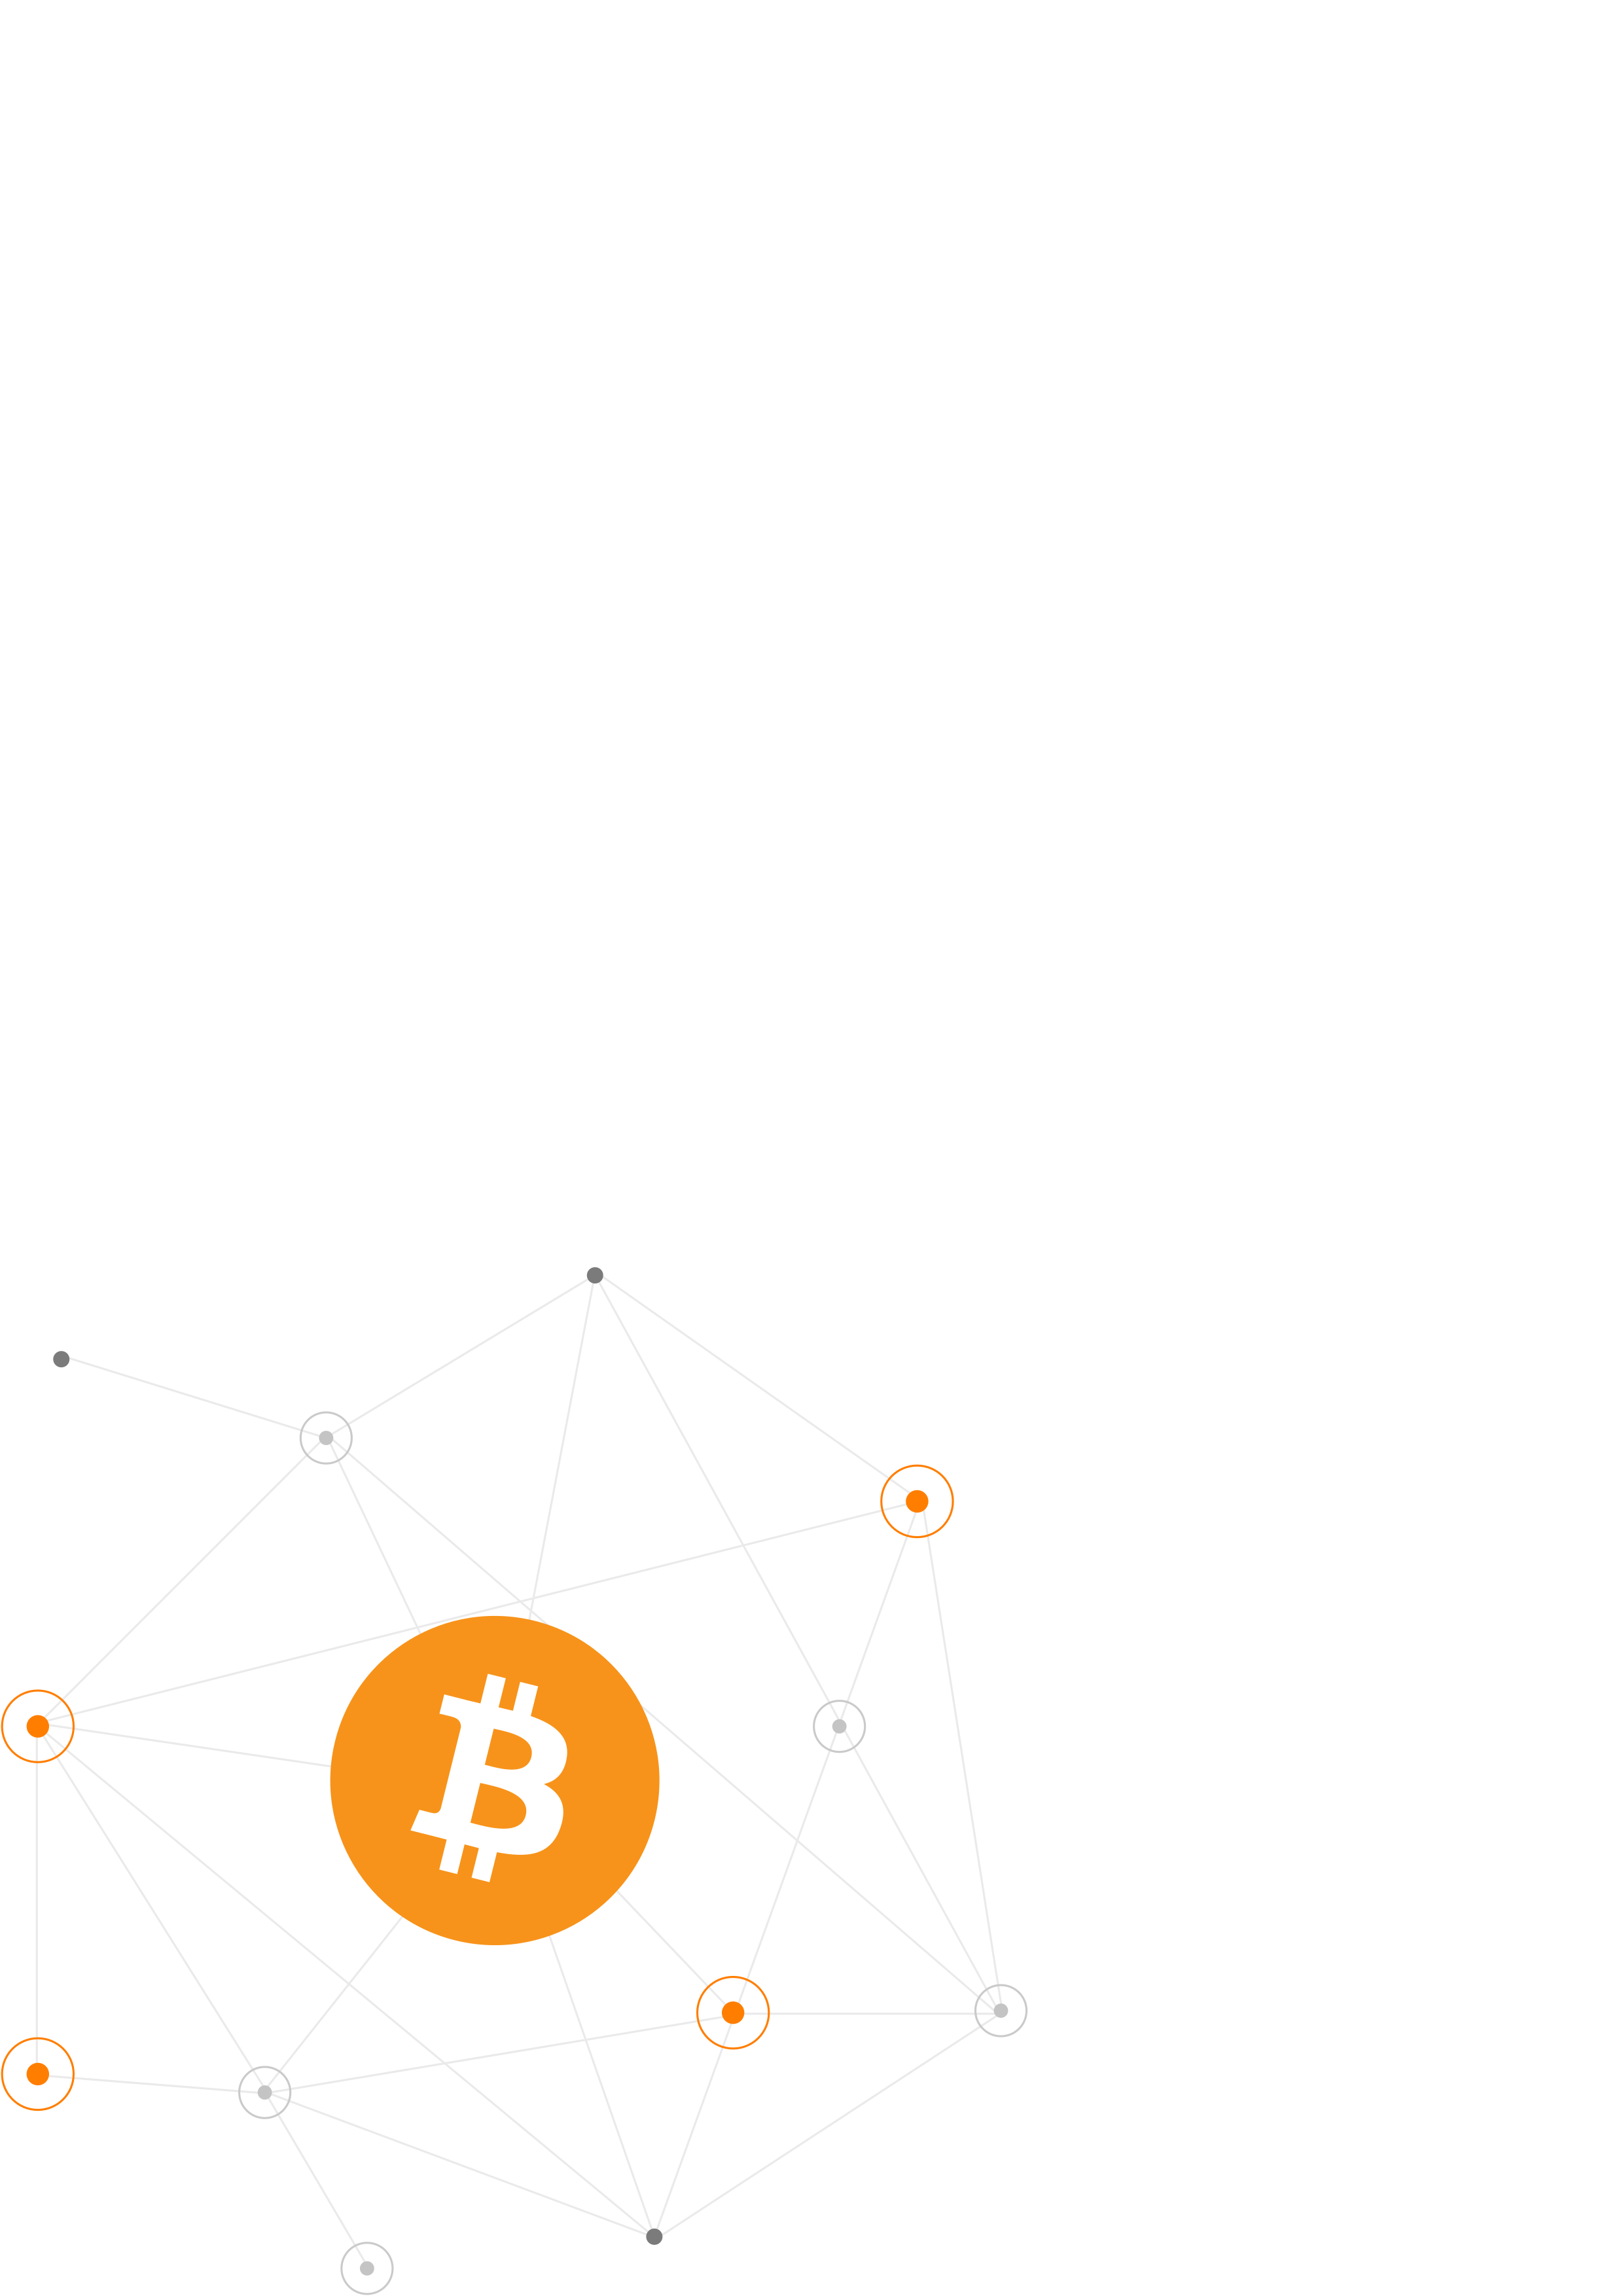
\includegraphics[height=3cm]{images/bitcoin-img.png}}
\title{\bitcoinA itcoin in Carnia}
\author{Eduardo Quintana-Miranda}
\date{04-11-2022}
\logo{
\includegraphics[height=0.5cm]{images/logotop.png}}

\begin{document}

\frame{\titlepage}

\begin{frame}
    \frametitle{Riassunto}
    \tableofcontents
\end{frame}

\section{Cosa \`e il \Bitcoin}
\begin{frame}{\insertsection}
    \centering
% - presentato al publico il 31 Ottobre 2008 e lanciato il 3 Gennaio 2009
% - open source
% - funziona usand un'insieme di regole matematiche scritte in codice e accetate
% per via di consenso
% - è denaro forte digitale, alcuni lo paragonano a oro: per la sua scarsita, durevole,
% verificabile, veloce, scalabile
% - sta portando la liberta economica alle persone in tutto il mondo,
% sopprattuto quelle che non hanno conti in banca:
%    non puo essere censurato, legato per nessuna legge o decisione politica
%    non puo essere sequestrato, o controllato per alcuna persona o governo
%    chiunque puo possiederlo ed usarlo, non importa dove abiti, quanti anni
%    hai, il colore della pelle, o lo stato legale, non importa neanche se sei un essere
%    umano, 
% - anche le machine possono inviare e ricevere bitcoin se gli si
%    programma per farlo.
%    non si ferma mai, ne weekend, ne giorni festivi, 
%    non puo essere hackerato, cancellato
%    costituisce la database piu sicura al mondo

    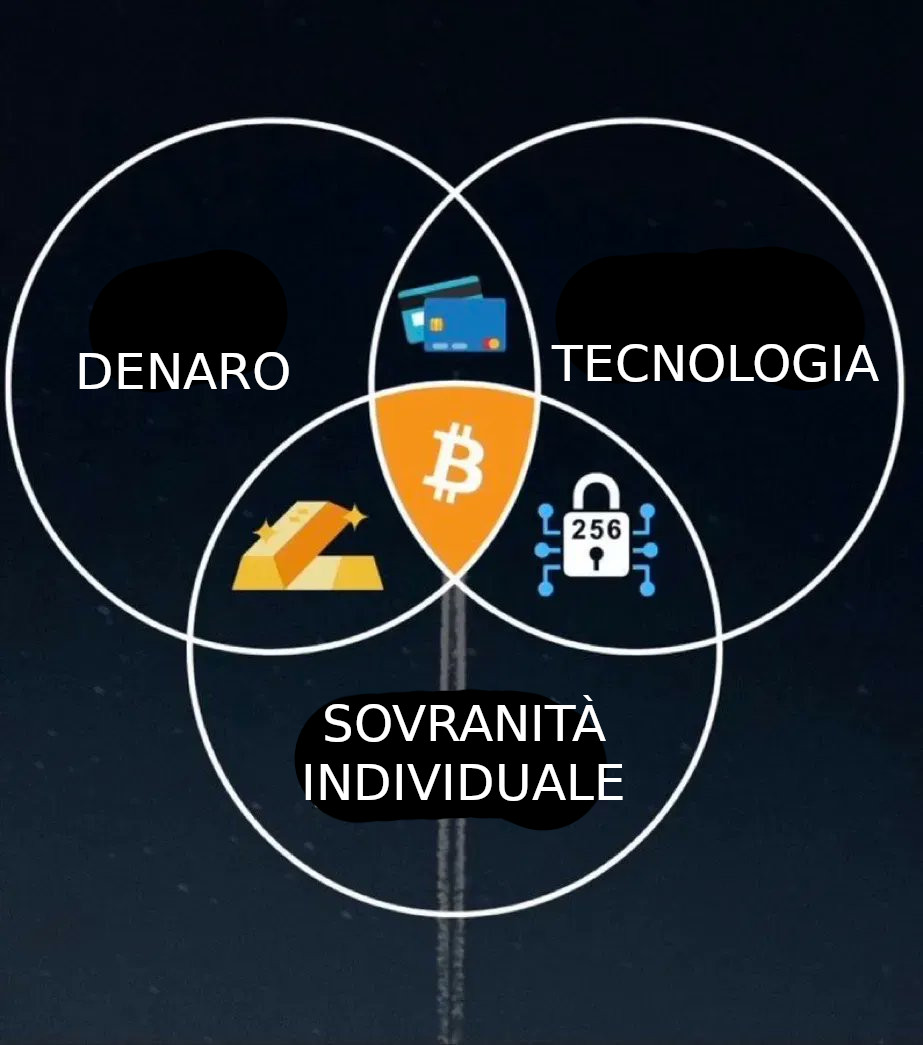
\includegraphics[height=.8\textheight]{images/money-technology-freedom-it.jpeg}
\end{frame}
\begin{frame}{\insertsection}
    \centering
% capire come funziona richiede di studio
% ma gli si puo usare in siccurezza dopo un paio di ore di educazione
% non 'e molto diverso da usare l'email o internet
    
\includegraphics[height=.8\textheight]{images/bitcoin-is-simple-it.jpeg}
\end{frame}

\section{Mining}
% bitcoin e un libro di contabilita publico, ogni transazione viene scritta in
% un blocco di dati e quei blochi vengono connessi e cosi ordinatin in sequenza
% portando una dimenzione causale nel mondo digitale.

% il mining 'e il processo di costruzione e inserimento dei blocchi a questa blockchain
% siccome 'e decentralizata, tutti i partecipanti (i minatori) devono
% collaborare per decidere cuale sara il prossimo blocco da aggiungere (questo
% sucede ogni 10 minuti).
% Per questo partecipano ad un concorso PoW, dove il vincitore (il primo che
% riesce a costruire un blocco valido) viene compensato con nuovi bitcoin + i
% costi delle transazioni (specie di mancia pagata dai debitori)

%    https://www.bitcoinmining.com/getting-started/
\begin{frame}{\insertsection}
    % What's mining and what's not. Why do we need energy.
    \begin{columns}
        \begin{column}{0.7\textwidth}
            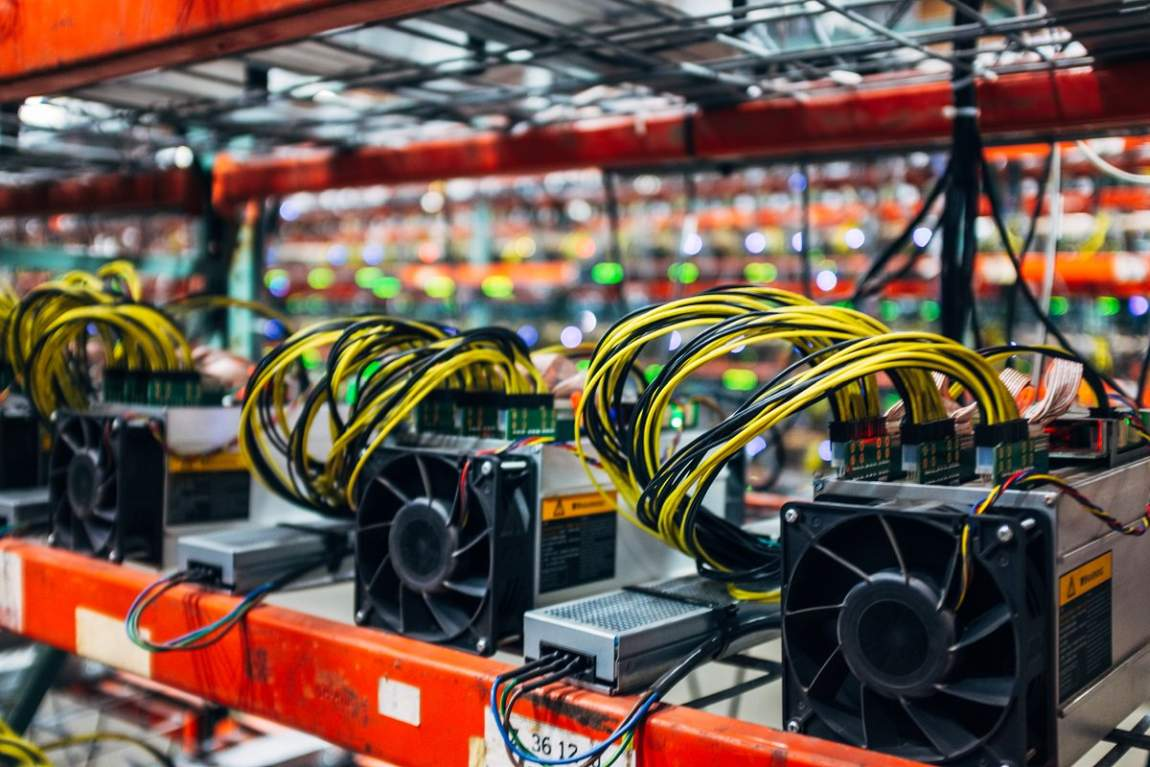
\includegraphics[width=\textwidth]{images/bitcoin-mining-pool.jpg}
        \end{column}
        \begin{column}{0.3\textwidth}
% un singolo CPU moderno puo calcolarni 70'000 di questi ogni secondo, e nel
% processo ne spenderesti 1MJ/Th,
% ci sono pero dei circuiti dedicate che ne calcono 100 Th/s (un milliardo di
% volte in piu) e spendono 21 J/Th (100 000 volte piu efficienti).
% Un singolo antiminer S19 pro certamente vuole una potenza di 3kW.
            \begin{block}{}
                \small
                \`E possible, ma inutile fare mining col PC.
            \end{block}
        \end{column}
    \end{columns}
\end{frame}

\section{Energia ed efficenza}

\begin{frame}{\insertsection}
\[
    E_{\mathrm{btc}}
    = E_h \frac{H_{\mathrm{world}} \cdot 10 \si{min}}{\mathrm{reward}}
    = 21\si{J/Th} \frac{250 \si{Eh/s} \cdot 10 \si{min}}{6.25 \mathrm{btc}}
\]
\[
    = 1,4 \times 10^5 \si{kWh}/\mathrm{btc}
\]
col prezzo attuale di mercato di circa $20 \si{k} \texteuro/\mathrm{btc}$
\[
    E_{\mathrm{btc}} \text{(equiv.)} 
    = 7 \si{kWh}/ \texteuro
\]
cioe $0,14 \texteuro / \si{kWh} $.

\visible<2>{
\begin{block}{}
    Il mining non \`e redditizio se si usa
    la energia della rete elettrica.
\end{block}}
\end{frame}

% Ef = 21 J/Th    // ASIC S19 XP efficiency
% Whr = 250 EH/s  // 1 Ex = 1000 Px = 1000'000 Tx
% reward_10min = 6.25 BTC
% Wh_10min = Whr * 600 s = 150'000 EH
% H_per_BTC = Wh_10min/reward_10min = 24'000 EH/BTC = 24 x 10^9 Th/BTC
% J_per_BTC = H_per_BTC * Ef = 504 x 10^9 J/BTC = 140 x 10^3 kWh / BTC

% if cost_electricity = 0.20 EUR / kWh
% equivalent cost of 1 BTC = J_per_BTC * cost_electricity = 28'000 EUR/BTC

% market price of BTC = 20'000 EUR/BTC
% or equivalently 0.14 EUR/kWh

\begin{frame}{\insertsection}
% nel contesto di questa presentazione, 'e importante sapere che questo concorso
% PoW diventa piu dificile se il potere di calcolo complessivo dei partecipanti
% cresce, in modo di avere sempre una media di 10min fra blocchi. Mentre che il
% compenso resta sempre quello. Per cui piu minatori ci sono, il guadagno
% aspettato diminuisce e i singoli devono valutare se la loro attivita economica
% e producente, perche sempre ci sono costi di hardware, manutenzione, e energia
% elettrica. Per legge di mercato, il margine di guadagno e spesso molto
% ridotto, e i minatori sono incentivati ad aumentare la efficienza energetica
% del loro hardware, e a trovare fonti di energia a basso costo, oppure gratis.

% la energia viene spessa nel computo ripetuto di una funzione matematica
% chiamata SHA256.


% dove va tutta questa energia?
% viene trasformata in calore dal effecto Joule
% quindi dal punto di vista di una persona che non vede cosa sta facendo questo
% circuito, ne vede della potenza fornita e della energia a forma di calore che
% ne emerge. lo stesso di una resistenza elettrica.

%    - the bottleneck of mining is in the SHA256 hash repeated computation, a single CPU can 
%    compute ? hashes per second, while some specialized chips can do ? hashes per second
%    and furthermore be more energy efficient (ie. hash computed per Joule of energy).
%    The current world hashrate is around 200 EH/s = 2*10^20 H/s approx 10 x 2^64 
%    (the number of wheat grains the inventor of chess wanted, but every 100ms)
%    
%    - still these machines consume energy
%    
%    ------(P)-----
%    |            |
%    ---[sha256]---
%    
%    for example the ant miner S9 consumes 1.5kW? at a hashrate of 1TH/s.
%    
%    - miner must weight the cost of electricity and hardware vs the possible gains from 
%    rewards. In the case of pools, the rewards is distributed across participants proportionally
%    to the hash rate of the contribuitors.
%    - very often the cost of electricity exceeds the value of the bitcoin at the moment of mining
%    
%    Cost-to-Mine-one-Bitcoin-Map.png
%    https://www.visualcapitalist.com/cp/the-cost-of-mining-bitcoin-in-198-different-countries/
%    
%    - in Italy for instance is $33k (current price $22k) TODO: update this numbers
%    
%    - having free energy like solar and wind is a must for most of us if we want to mine
%    
%    - but where is all this energy going? question to the public
%    
%    - by energy conservation law these system produce heat at a rate of P.
%    
%    - is this a waste of energy? 
\begin{columns}
    \begin{column}{.5\textwidth}
    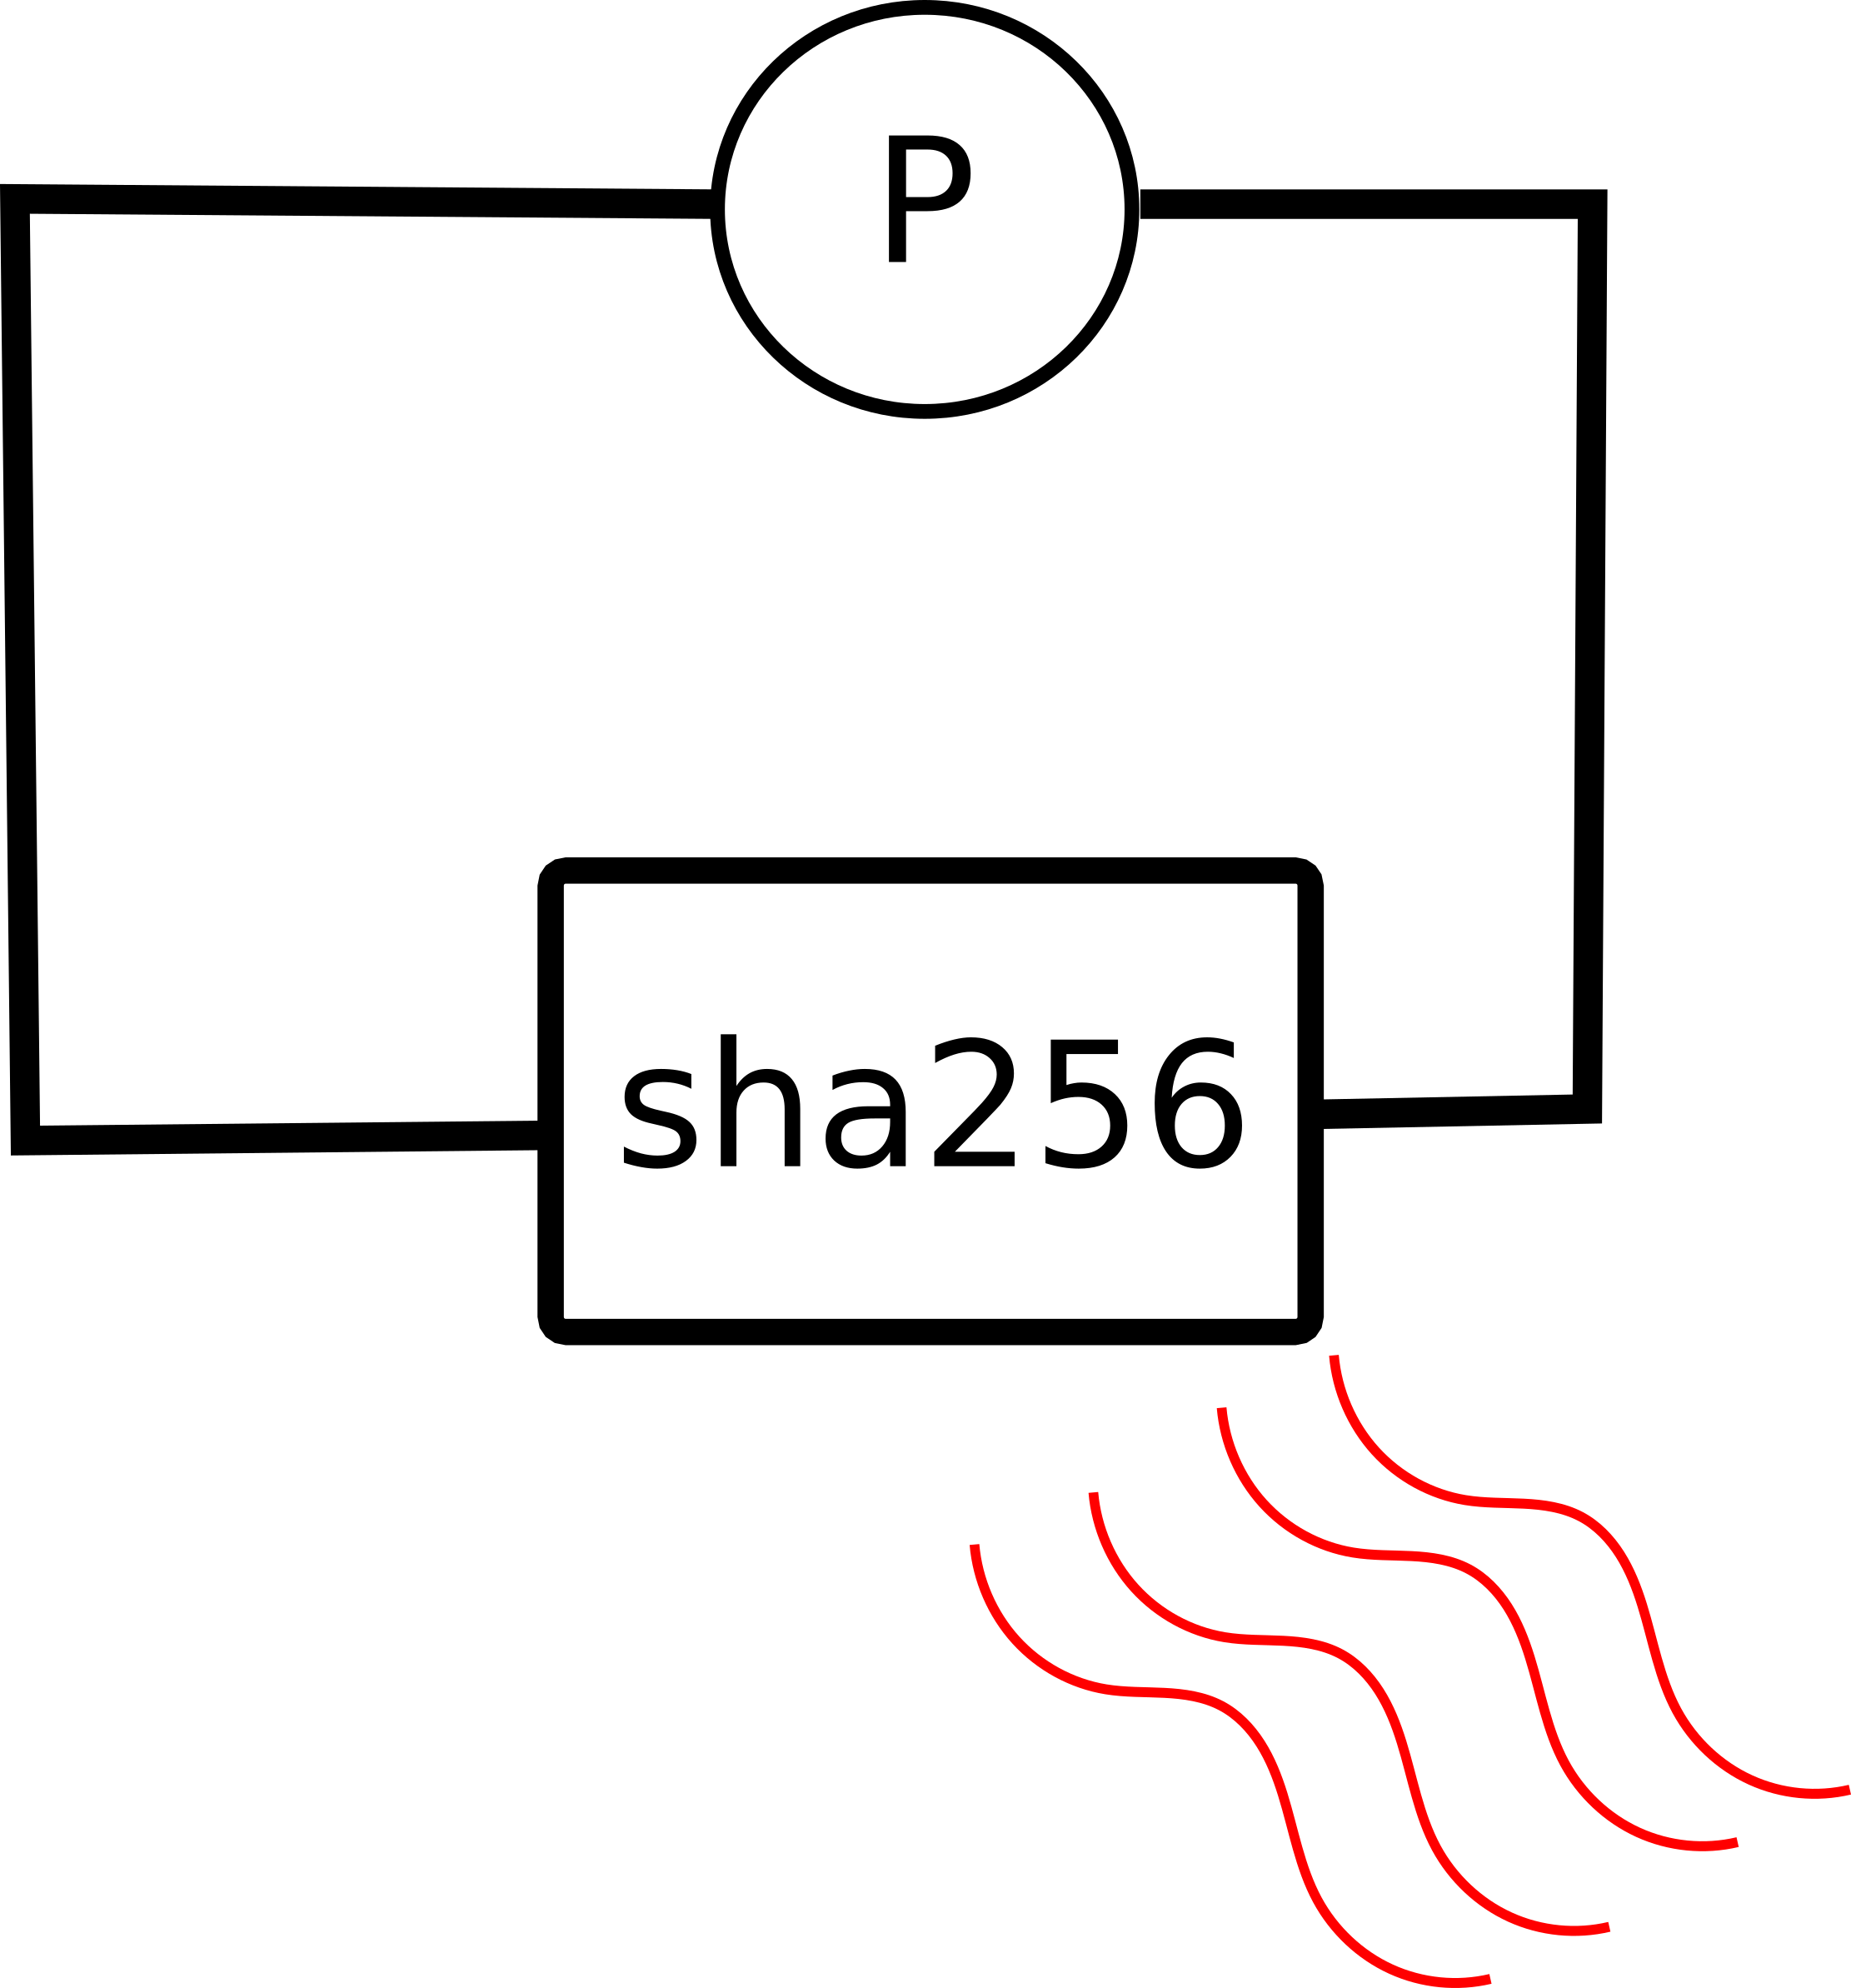
\includegraphics[width=\textwidth]{images/sha256-heat.png}
    \end{column}
    \begin{column}{.5\textwidth}
       \begin{block}{}
       La energia impiegata viene rilasciata come calore.
       \end{block}
    \end{column}
\end{columns}
\end{frame}

\section{Idea per startup}
\begin{frame}{Calore con e senza Calcolo}
    \centering
% Imaginiamo la seguente situazione, due circuiti uno Sha256 e l'altro
% semplicemente una resistenza. Se i due consumano la stessa potenza P (nel
% intervallo da 1kW o 500W) propio come una stuffeta elettrica o uno scaldabagno.

% - alla sinistra abbiamo Alice che usa della elettricita per scaldare la sua
% casa
% - mentre che alla destra abbiamo Bob, che ne usa la stessa quantita di energia
% elettrica per partecipare al PoW (guadagnandosi dei bitcoin) e nel mentre si
% scalda la casa.

% per la legge di conservazione della energia entrambi circuiti consumano la
% stessa quantita di energia elettrica ed entrambi rilascerano la
% stessa quantita di calore. Ma Bob ne fa un uso piu efficiente di quella
% energia.
    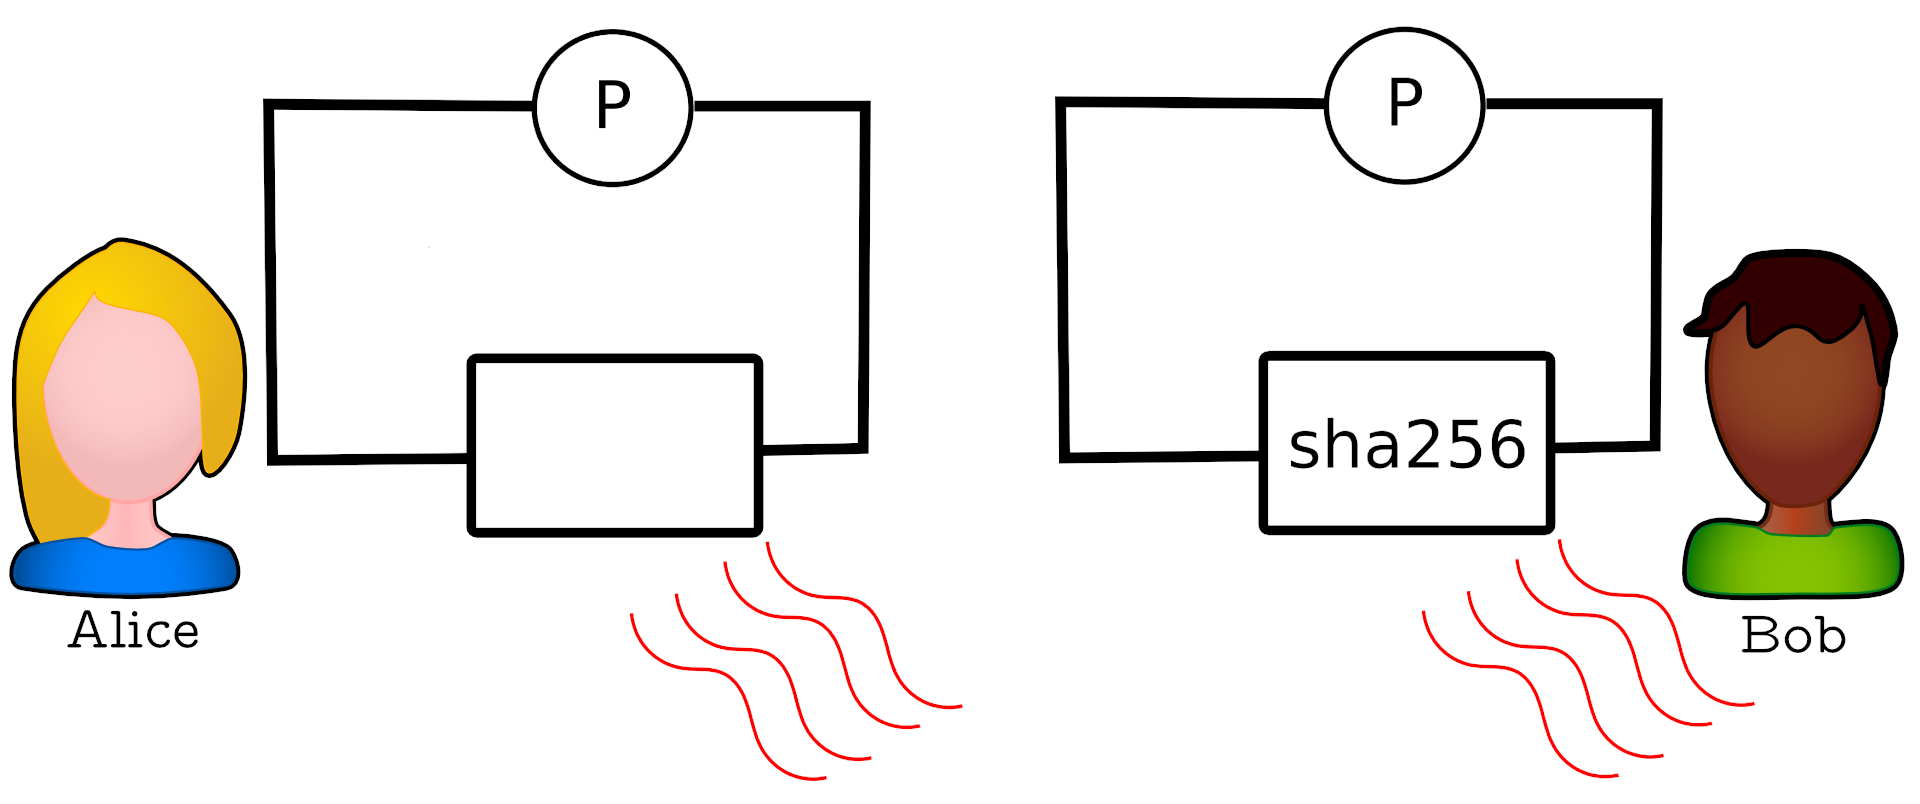
\includegraphics[height=.5\textheight]{images/alice-bob.png}
\visible<2>{\begin{block}{}
Non spendiamo pi\`u energia per mining, usiamo il mining per pagare
la energia che utiliziamo.
\end{block}}
\end{frame}

% Cryptographic security, censorship resistance
\begin{frame}{Accumulo calore \Bitcoin}
    \centering
    % Can \Bitcoin\ be hacked, censored, controlled, stopped?
    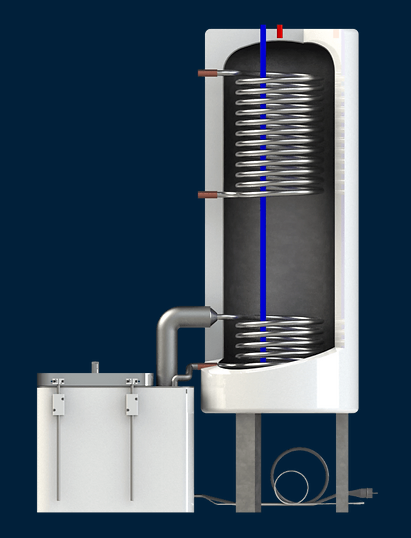
\includegraphics[height=.8\textheight]{images/sato.png}\footnote{\url{https://www.wisemining.io/}}\quad
\end{frame}


\begin{frame}{Competitori nel Mercato}
    \centering
    % ci sono i competitore nel mercato, ma sono pocchi e quindi i prezzi sono
    % elevati piu le tasse di importazione.
    
    % l'idea sarebbe di iniziare una azienda di ricerca e svilupo di questi
    % hardware per mining casalinghi in Italia. I consumatori potrebbero vedere
    % questa opportunita per abassare il costo delle bollete, e contribuire alla
    % decentralizazione della rete Bitcoin.
    
    % 
\includegraphics[height=.1\textheight]{images/heatbit-logo.png}
    % 
\includegraphics[height=.05\textheight]{images/us.png}
    % 
\includegraphics[height=.1\textheight]{images/wisemining-logo.png}
    % 
\includegraphics[height=.1\textheight]{images/ming-energy-logo.png}
    
    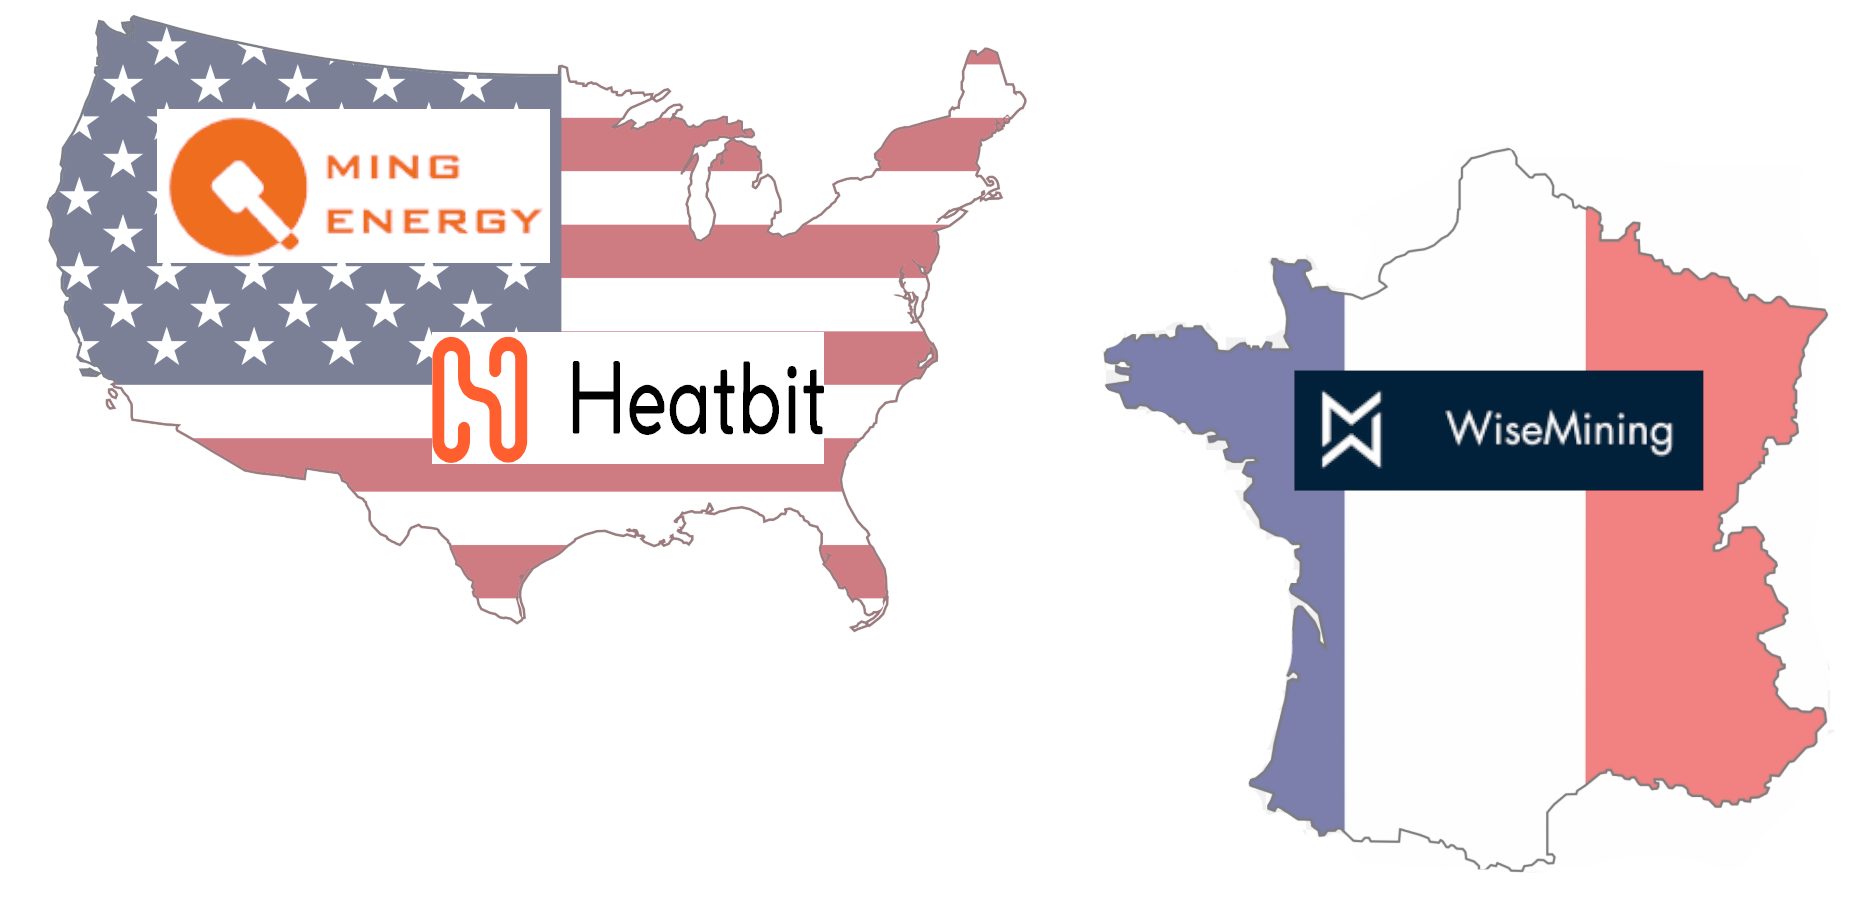
\includegraphics[width=\textwidth]{images/competitors.png}
    
    \phantom{\footnote{\url{https://www.heatbit.com/}}}
    \phantom{\footnote{\url{https://www.wisemining.io/}}}
    \phantom{\footnote{\url{https://bitcoinminingheater.com/}}}
\end{frame}

\begin{frame}{Parole finali}
    \centering
    % per concludere vorrei lasciarvi un meme molto noto, con un messagio
    % profondo: Bitcoin e piu di un bene con un valore di mercato destinato a
    % valere millioni di dollari un giorno. 
    % 'E anche una alternativa al sistema finanziario centralizzato.
    % Le previsioni degli intusiasti (io compresso) che nel futuro il bitcoin
    % sara omnipresente. Forse i bambini che nascono oggi quando avranno l'eta
    % richiesta per aprire un conto in banca, gia non ne avranno bisogno, perche
    % potranno essere loro stessi i propi banchieri tramite un app nel
    % telefonino e potrano ricevere bitcoin come stipendio e pagare in bitcoin
    % ai comerciante per beni e servizi.
    
\includegraphics[height=.8\textheight]{images/matrix-1M-it.jpeg}
\end{frame}

\begin{frame}{Per saperne di pi\`u}
    \centering
    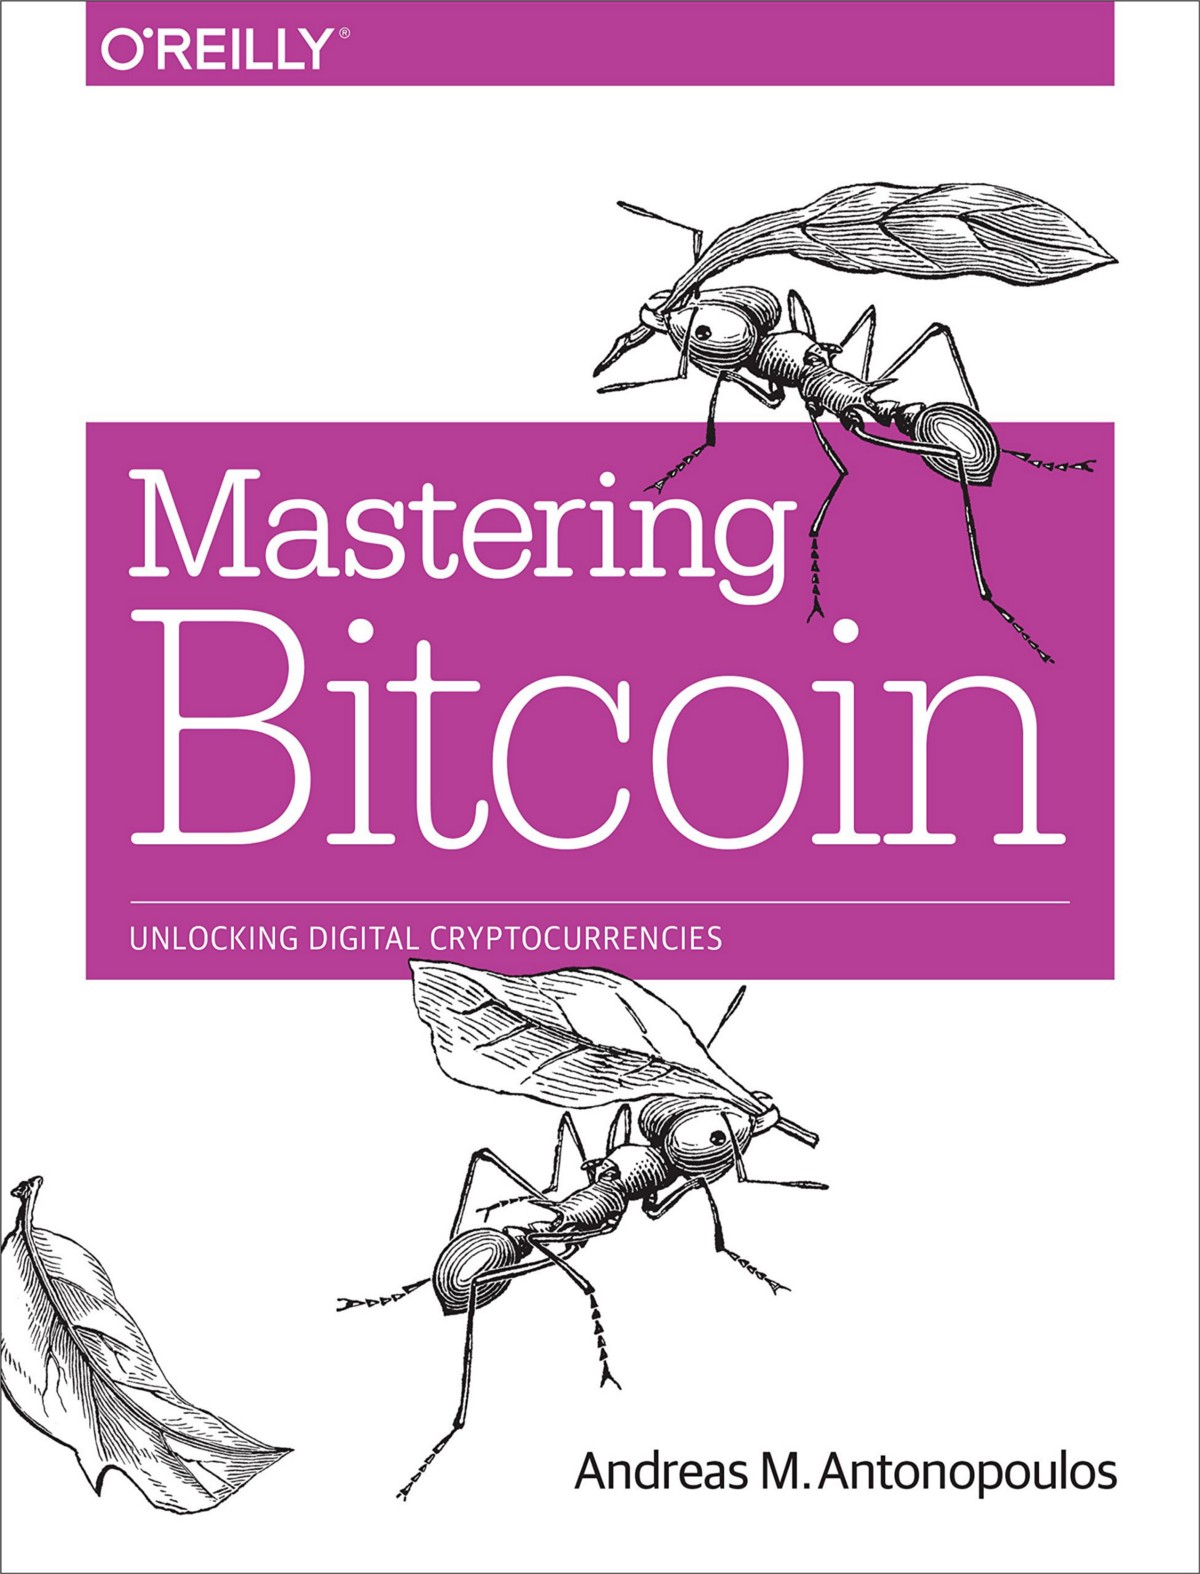
\includegraphics[width=.3\textwidth]{images/mastering-bitcoin.jpeg}\quad
    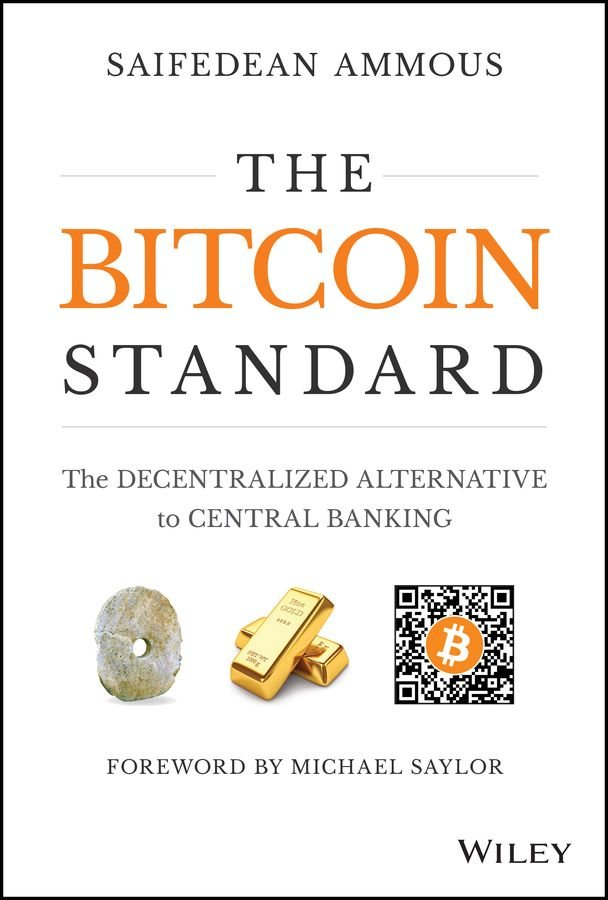
\includegraphics[width=.3\textwidth]{images/bitcoin-standard.jpeg}
\end{frame}

\end{document}
